\section{Environment}
The Danish Medical Association (DMA) is an association that aims to represent the entire Danish medical sector and its existing organisations, tying them all together and providing benefits for all its members. There are three major medical organisations under the DMA. The structure is illustrated in figure \ref{dmaorganisation}.

The first is “Yngre Læger” (YL), an association for younger doctors with close ties to doctors advancing their studies in the “klinisk basisuddannelse” (KBU), those taking their introduction to their speciality and those who are actively specialising.

The second is “Forening af Speciallæger” (FAS) which is a union for consulting doctors that have studied a speciality.

Lastly is “Praktiserende Lægers Organisation” (PLO) which is an organisation for the practicioning family doctors who usually run their own local clinic for the nearby population.

Danish doctors are generally associated with one of these three organisations and are thus members of the DMA, having access to the DMA provided courses and other benefits.

\begin{figure*}[h!]
 \begin{center}
  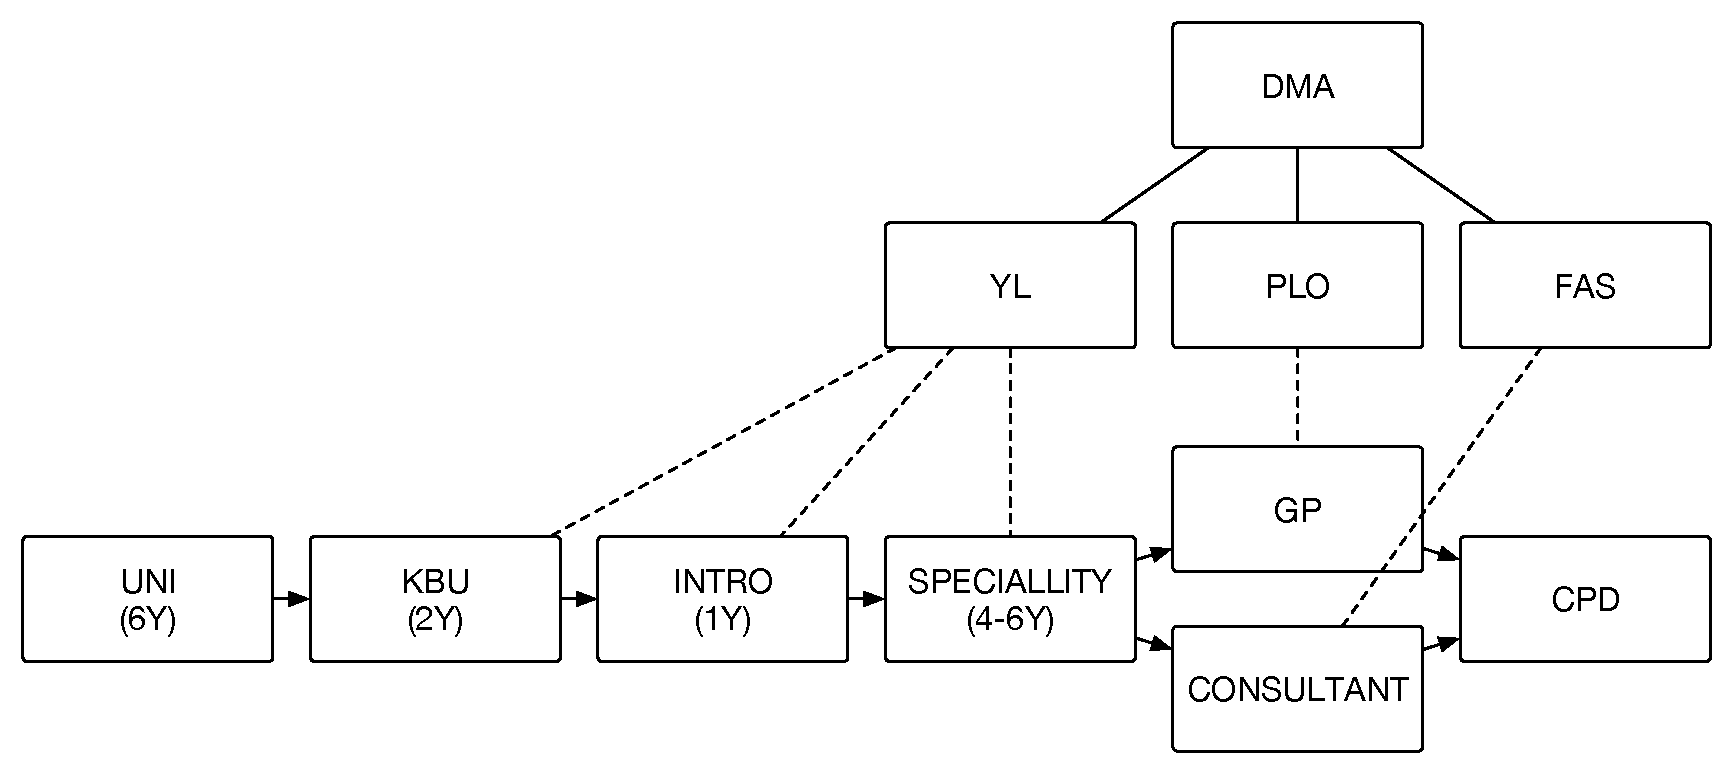
\includegraphics[width=1\textwidth]{figures/dma-structure.pdf}
  \caption{The structure of the DMA organisation.\label{dmaorganisation}}
 \end{center}
\end{figure*}

\subsection{Potential and needs}
DMA members need to take courses in order to stay up to date with the latest information about medicine. So far the existing e-learning platforms that provide the necessary courses are not widely used by the doctors, in some cases this is because they consider it to be time consuming. Some doctors also consider the contents of the e-learning courses to be too easy and superficial.. What is needed is a new way to deliver information to the doctors, such that we can engage the doctors in a way that eliminates the concerns of the current e-learning solutions.

\subsection{Requirements and conditions}
DMA members are looking for a new e-learning platform with a different approach compared to the existing offers provided by DMA, such as BMJ Learning as the DMA members currently do not utilise the offers as much as expected. DMA would like to have the content focused on including the entire spectrum (known as the 7 roles of physicians) of knowledge areas which a modern doctor should be educated in, for example there should be topics dealing with communication, administration and so on. Currently surveys performed by DMA show that some doctors prefer to strictly focus their education on medical expertise and entirely neglecting being educated in the remaining 6 roles.

\subsection{Special conditions}
We do not identify any special conditions at this point.

